\documentclass[twoside]{book}

% Packages required by doxygen
\usepackage{fixltx2e}
\usepackage{calc}
\usepackage{doxygen}
\usepackage{graphicx}
\usepackage[utf8]{inputenc}
\usepackage{makeidx}
\usepackage{multicol}
\usepackage{multirow}
\PassOptionsToPackage{warn}{textcomp}
\usepackage{textcomp}
\usepackage[nointegrals]{wasysym}
\usepackage[table]{xcolor}

% Font selection
\usepackage[T1]{fontenc}
\usepackage{mathptmx}
\usepackage[scaled=.90]{helvet}
\usepackage{courier}
\usepackage{amssymb}
\usepackage{sectsty}
\renewcommand{\familydefault}{\sfdefault}
\allsectionsfont{%
  \fontseries{bc}\selectfont%
  \color{darkgray}%
}
\renewcommand{\DoxyLabelFont}{%
  \fontseries{bc}\selectfont%
  \color{darkgray}%
}
\newcommand{\+}{\discretionary{\mbox{\scriptsize$\hookleftarrow$}}{}{}}

% Page & text layout
\usepackage{geometry}
\geometry{%
  a4paper,%
  top=2.5cm,%
  bottom=2.5cm,%
  left=2.5cm,%
  right=2.5cm%
}
\tolerance=750
\hfuzz=15pt
\hbadness=750
\setlength{\emergencystretch}{15pt}
\setlength{\parindent}{0cm}
\setlength{\parskip}{0.2cm}
\makeatletter
\renewcommand{\paragraph}{%
  \@startsection{paragraph}{4}{0ex}{-1.0ex}{1.0ex}{%
    \normalfont\normalsize\bfseries\SS@parafont%
  }%
}
\renewcommand{\subparagraph}{%
  \@startsection{subparagraph}{5}{0ex}{-1.0ex}{1.0ex}{%
    \normalfont\normalsize\bfseries\SS@subparafont%
  }%
}
\makeatother

% Headers & footers
\usepackage{fancyhdr}
\pagestyle{fancyplain}
\fancyhead[LE]{\fancyplain{}{\bfseries\thepage}}
\fancyhead[CE]{\fancyplain{}{}}
\fancyhead[RE]{\fancyplain{}{\bfseries\leftmark}}
\fancyhead[LO]{\fancyplain{}{\bfseries\rightmark}}
\fancyhead[CO]{\fancyplain{}{}}
\fancyhead[RO]{\fancyplain{}{\bfseries\thepage}}
\fancyfoot[LE]{\fancyplain{}{}}
\fancyfoot[CE]{\fancyplain{}{}}
\fancyfoot[RE]{\fancyplain{}{\bfseries\scriptsize Generated on Tue Mar 28 2017 10\+:18\+:29 for drunk\+\_\+player by Doxygen }}
\fancyfoot[LO]{\fancyplain{}{\bfseries\scriptsize Generated on Tue Mar 28 2017 10\+:18\+:29 for drunk\+\_\+player by Doxygen }}
\fancyfoot[CO]{\fancyplain{}{}}
\fancyfoot[RO]{\fancyplain{}{}}
\renewcommand{\footrulewidth}{0.4pt}
\renewcommand{\chaptermark}[1]{%
  \markboth{#1}{}%
}
\renewcommand{\sectionmark}[1]{%
  \markright{\thesection\ #1}%
}

% Indices & bibliography
\usepackage{natbib}
\usepackage[titles]{tocloft}
\setcounter{tocdepth}{3}
\setcounter{secnumdepth}{5}
\makeindex

% Hyperlinks (required, but should be loaded last)
\usepackage{ifpdf}
\ifpdf
  \usepackage[pdftex,pagebackref=true]{hyperref}
\else
  \usepackage[ps2pdf,pagebackref=true]{hyperref}
\fi
\hypersetup{%
  colorlinks=true,%
  linkcolor=blue,%
  citecolor=blue,%
  unicode%
}

% Custom commands
\newcommand{\clearemptydoublepage}{%
  \newpage{\pagestyle{empty}\cleardoublepage}%
}


%===== C O N T E N T S =====

\begin{document}

% Titlepage & ToC
\hypersetup{pageanchor=false,
             bookmarks=true,
             bookmarksnumbered=true,
             pdfencoding=unicode
            }
\pagenumbering{roman}
\begin{titlepage}
\vspace*{7cm}
\begin{center}%
{\Large drunk\+\_\+player }\\
\vspace*{1cm}
{\large Generated by Doxygen 1.8.8}\\
\vspace*{0.5cm}
{\small Tue Mar 28 2017 10:18:29}\\
\end{center}
\end{titlepage}
\clearemptydoublepage
\tableofcontents
\clearemptydoublepage
\pagenumbering{arabic}
\hypersetup{pageanchor=true}

%--- Begin generated contents ---
\chapter{Documentation de drunk\+\_\+player}
\label{index}\hypertarget{index}{}Drunk\+\_\+player est un système de lecture de vidéos qui a trop bu. Il lit les vidéos contenues dans un dossier par morceaux, aléatoirement et parfois en transformant l'image. Drunk\+\_\+player utilise la bibliothèque de traitement d'image Open\+C\+V et est composé \+:


\begin{DoxyItemize}
\item d'une bibliothèque (drunk\+\_\+player) contenant le code de base
\item d'un programme graphique (drunk\+\_\+player\+\_\+gui) qui affiche le résultat à l'écran
\item d'un programme console (drunk\+\_\+player\+\_\+cli) qui sort le résultat dans un fichier 
\end{DoxyItemize}
\chapter{Todo List}
\label{todo}
\hypertarget{todo}{}

\begin{DoxyRefList}
\item[\label{todo__todo000001}%
\hypertarget{todo__todo000001}{}%
Member \hyperlink{classChrono_a027be23720616639bc610a98c53740ea}{Chrono\+:\+:reset} ()]Remet la mesure à zéro. Ne change pas l'état démarré/arrêté du chronomètre. 
\end{DoxyRefList}
\chapter{Bug List}
\label{bug}
\hypertarget{bug}{}

\begin{DoxyRefList}
\item[\label{bug__bug000001}%
\hypertarget{bug__bug000001}{}%
Class \hyperlink{classAbstractPlayer}{Abstract\+Player} ]\+: le son n'est pas géré 
\end{DoxyRefList}
\chapter{Hierarchical Index}
\section{Class Hierarchy}
This inheritance list is sorted roughly, but not completely, alphabetically\+:\begin{DoxyCompactList}
\item \contentsline{section}{Abstract\+Player}{\pageref{classAbstractPlayer}}{}
\begin{DoxyCompactList}
\item \contentsline{section}{Drunk\+Player}{\pageref{classDrunkPlayer}}{}
\end{DoxyCompactList}
\item \contentsline{section}{Chrono}{\pageref{classChrono}}{}
\item \contentsline{section}{Random}{\pageref{classRandom}}{}
\end{DoxyCompactList}

\chapter{Class Index}
\section{Class List}
Here are the classes, structs, unions and interfaces with brief descriptions\+:\begin{DoxyCompactList}
\item\contentsline{section}{\hyperlink{classAbstractPlayer}{Abstract\+Player} }{\pageref{classAbstractPlayer}}{}
\item\contentsline{section}{\hyperlink{classChrono}{Chrono} \\*Chronomètre pour mesurer des durées. Exemple d'utilisation \+: \hyperlink{classChrono}{Chrono} chrono; chrono.\+start(); ... chrono.\+stop(); std\+::cout $<$$<$ \char`\"{}temps écoulé \+: \char`\"{} $<$$<$ chrono.\+elapsed() $<$$<$ std\+::endl; }{\pageref{classChrono}}{}
\item\contentsline{section}{\hyperlink{classDrunkPlayer}{Drunk\+Player} \\*Lecteur vidéo qui lit des vidéos par morceaux désordonnés et transformés }{\pageref{classDrunkPlayer}}{}
\item\contentsline{section}{\hyperlink{classRandom}{Random} }{\pageref{classRandom}}{}
\end{DoxyCompactList}

\chapter{File Index}
\section{File List}
Here is a list of all files with brief descriptions\+:\begin{DoxyCompactList}
\item\contentsline{section}{/etudiants/asmlali/\+G\+L/\+L3\+\_\+\+G\+L\+\_\+etudiant/\+T\+P\+\_\+documentation/drunk\+\_\+player/src/\hyperlink{mainpage_8hpp}{mainpage.\+hpp} }{\pageref{mainpage_8hpp}}{}
\item\contentsline{section}{/etudiants/asmlali/\+G\+L/\+L3\+\_\+\+G\+L\+\_\+etudiant/\+T\+P\+\_\+documentation/drunk\+\_\+player/src/drunk\+\_\+player/\hyperlink{Chrono_8cpp}{Chrono.\+cpp} }{\pageref{Chrono_8cpp}}{}
\item\contentsline{section}{/etudiants/asmlali/\+G\+L/\+L3\+\_\+\+G\+L\+\_\+etudiant/\+T\+P\+\_\+documentation/drunk\+\_\+player/src/drunk\+\_\+player/\hyperlink{Chrono_8hpp}{Chrono.\+hpp} }{\pageref{Chrono_8hpp}}{}
\item\contentsline{section}{/etudiants/asmlali/\+G\+L/\+L3\+\_\+\+G\+L\+\_\+etudiant/\+T\+P\+\_\+documentation/drunk\+\_\+player/src/drunk\+\_\+player/\hyperlink{Filesystem_8cpp}{Filesystem.\+cpp} }{\pageref{Filesystem_8cpp}}{}
\item\contentsline{section}{/etudiants/asmlali/\+G\+L/\+L3\+\_\+\+G\+L\+\_\+etudiant/\+T\+P\+\_\+documentation/drunk\+\_\+player/src/drunk\+\_\+player/\hyperlink{Filesystem_8hpp}{Filesystem.\+hpp} }{\pageref{Filesystem_8hpp}}{}
\item\contentsline{section}{/etudiants/asmlali/\+G\+L/\+L3\+\_\+\+G\+L\+\_\+etudiant/\+T\+P\+\_\+documentation/drunk\+\_\+player/src/drunk\+\_\+player/\hyperlink{Player_8cpp}{Player.\+cpp} }{\pageref{Player_8cpp}}{}
\item\contentsline{section}{/etudiants/asmlali/\+G\+L/\+L3\+\_\+\+G\+L\+\_\+etudiant/\+T\+P\+\_\+documentation/drunk\+\_\+player/src/drunk\+\_\+player/\hyperlink{Player_8hpp}{Player.\+hpp} }{\pageref{Player_8hpp}}{}
\item\contentsline{section}{/etudiants/asmlali/\+G\+L/\+L3\+\_\+\+G\+L\+\_\+etudiant/\+T\+P\+\_\+documentation/drunk\+\_\+player/src/drunk\+\_\+player/\hyperlink{Random_8cpp}{Random.\+cpp} }{\pageref{Random_8cpp}}{}
\item\contentsline{section}{/etudiants/asmlali/\+G\+L/\+L3\+\_\+\+G\+L\+\_\+etudiant/\+T\+P\+\_\+documentation/drunk\+\_\+player/src/drunk\+\_\+player/\hyperlink{Random_8hpp}{Random.\+hpp} }{\pageref{Random_8hpp}}{}
\item\contentsline{section}{/etudiants/asmlali/\+G\+L/\+L3\+\_\+\+G\+L\+\_\+etudiant/\+T\+P\+\_\+documentation/drunk\+\_\+player/src/drunk\+\_\+player\+\_\+cli/\hyperlink{drunk__player__cli_8cpp}{drunk\+\_\+player\+\_\+cli.\+cpp} }{\pageref{drunk__player__cli_8cpp}}{}
\item\contentsline{section}{/etudiants/asmlali/\+G\+L/\+L3\+\_\+\+G\+L\+\_\+etudiant/\+T\+P\+\_\+documentation/drunk\+\_\+player/src/drunk\+\_\+player\+\_\+gui/\hyperlink{drunk__player__gui_8cpp}{drunk\+\_\+player\+\_\+gui.\+cpp} }{\pageref{drunk__player__gui_8cpp}}{}
\end{DoxyCompactList}

\chapter{Class Documentation}
\hypertarget{classAbstractPlayer}{\section{Abstract\+Player Class Reference}
\label{classAbstractPlayer}\index{Abstract\+Player@{Abstract\+Player}}
}


{\ttfamily \#include $<$Player.\+hpp$>$}



Inheritance diagram for Abstract\+Player\+:\nopagebreak
\begin{figure}[H]
\begin{center}
\leavevmode
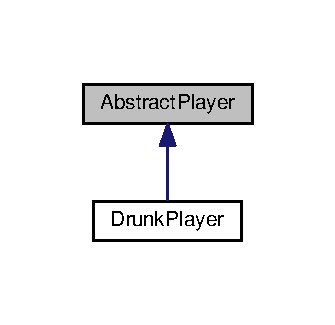
\includegraphics[width=161pt]{classAbstractPlayer__inherit__graph}
\end{center}
\end{figure}
\subsection*{Public Member Functions}
\begin{DoxyCompactItemize}
\item 
\hyperlink{classAbstractPlayer_a4987602a4b3381a9c592585dde7cf33b}{Abstract\+Player} ()
\begin{DoxyCompactList}\small\item\em Classe abstraite de base pour des lecteurs vidéo. \end{DoxyCompactList}\item 
virtual void \hyperlink{classAbstractPlayer_a2091b1757bfd13116dfa4612af55473b}{load\+Folder} (const std\+::string \&folder\+Name)
\item 
int \hyperlink{classAbstractPlayer_a8bdc017fb32c90e6635ed6b7491fbe98}{get\+Image\+Size} () const 
\item 
virtual bool \hyperlink{classAbstractPlayer_a841896a599ebe6b8317905de78c44bcc}{is\+Finished} () const =0
\begin{DoxyCompactList}\small\item\em Retourne si toutes les vidéos ont été lues entièrement. \end{DoxyCompactList}\item 
virtual void \hyperlink{classAbstractPlayer_a5c9a863c96224dd297aa44c69010cd94}{operator$>$$>$} (cv\+::\+Mat \&image)=0
\begin{DoxyCompactList}\small\item\em Lit une image du flux vidéo. \end{DoxyCompactList}\end{DoxyCompactItemize}
\subsection*{Protected Attributes}
\begin{DoxyCompactItemize}
\item 
std\+::vector$<$ cv\+::\+Video\+Capture $>$ \hyperlink{classAbstractPlayer_a72dd2ef25310decd45671a7d51e1f319}{\+\_\+captures}
\item 
int \hyperlink{classAbstractPlayer_a9d8395a141cc985622d4910209bc7d53}{\+\_\+size}
\end{DoxyCompactItemize}


\subsection{Detailed Description}
Lecteur de video (classe abstraite). todo \+: implémenter un lecteur classique qui lit toutes les vidéos à la suite \begin{DoxyRefDesc}{Bug}
\item[\hyperlink{bug__bug000001}{Bug}]\+: le son n'est pas géré \end{DoxyRefDesc}


\subsection{Constructor \& Destructor Documentation}
\hypertarget{classAbstractPlayer_a4987602a4b3381a9c592585dde7cf33b}{\index{Abstract\+Player@{Abstract\+Player}!Abstract\+Player@{Abstract\+Player}}
\index{Abstract\+Player@{Abstract\+Player}!Abstract\+Player@{Abstract\+Player}}
\subsubsection[{Abstract\+Player}]{\setlength{\rightskip}{0pt plus 5cm}Abstract\+Player\+::\+Abstract\+Player (
\begin{DoxyParamCaption}
{}
\end{DoxyParamCaption}
)}}\label{classAbstractPlayer_a4987602a4b3381a9c592585dde7cf33b}


Classe abstraite de base pour des lecteurs vidéo. 



\subsection{Member Function Documentation}
\hypertarget{classAbstractPlayer_a8bdc017fb32c90e6635ed6b7491fbe98}{\index{Abstract\+Player@{Abstract\+Player}!get\+Image\+Size@{get\+Image\+Size}}
\index{get\+Image\+Size@{get\+Image\+Size}!Abstract\+Player@{Abstract\+Player}}
\subsubsection[{get\+Image\+Size}]{\setlength{\rightskip}{0pt plus 5cm}int Abstract\+Player\+::get\+Image\+Size (
\begin{DoxyParamCaption}
{}
\end{DoxyParamCaption}
) const}}\label{classAbstractPlayer_a8bdc017fb32c90e6635ed6b7491fbe98}
Retourne la taille maximale des vidéos. Ne distingue pas largeur/hauteur. \hypertarget{classAbstractPlayer_a841896a599ebe6b8317905de78c44bcc}{\index{Abstract\+Player@{Abstract\+Player}!is\+Finished@{is\+Finished}}
\index{is\+Finished@{is\+Finished}!Abstract\+Player@{Abstract\+Player}}
\subsubsection[{is\+Finished}]{\setlength{\rightskip}{0pt plus 5cm}virtual bool Abstract\+Player\+::is\+Finished (
\begin{DoxyParamCaption}
{}
\end{DoxyParamCaption}
) const\hspace{0.3cm}{\ttfamily [pure virtual]}}}\label{classAbstractPlayer_a841896a599ebe6b8317905de78c44bcc}


Retourne si toutes les vidéos ont été lues entièrement. 



Implemented in \hyperlink{classDrunkPlayer_a9c032dda7df01fafc757fb1f4e265bb4}{Drunk\+Player}.

\hypertarget{classAbstractPlayer_a2091b1757bfd13116dfa4612af55473b}{\index{Abstract\+Player@{Abstract\+Player}!load\+Folder@{load\+Folder}}
\index{load\+Folder@{load\+Folder}!Abstract\+Player@{Abstract\+Player}}
\subsubsection[{load\+Folder}]{\setlength{\rightskip}{0pt plus 5cm}void Abstract\+Player\+::load\+Folder (
\begin{DoxyParamCaption}
\item[{const std\+::string \&}]{folder\+Name}
\end{DoxyParamCaption}
)\hspace{0.3cm}{\ttfamily [virtual]}}}\label{classAbstractPlayer_a2091b1757bfd13116dfa4612af55473b}
Lit tous les fichiers d'un dossier. precondition \+: considère que les fichiers sont tous des vidéos exception \+: std\+::string si pas de fichiers valides 

Reimplemented in \hyperlink{classDrunkPlayer_a235e60ea8a97c4d26277b066c2cebe80}{Drunk\+Player}.

\hypertarget{classAbstractPlayer_a5c9a863c96224dd297aa44c69010cd94}{\index{Abstract\+Player@{Abstract\+Player}!operator$>$$>$@{operator$>$$>$}}
\index{operator$>$$>$@{operator$>$$>$}!Abstract\+Player@{Abstract\+Player}}
\subsubsection[{operator$>$$>$}]{\setlength{\rightskip}{0pt plus 5cm}virtual void Abstract\+Player\+::operator$>$$>$ (
\begin{DoxyParamCaption}
\item[{cv\+::\+Mat \&}]{image}
\end{DoxyParamCaption}
)\hspace{0.3cm}{\ttfamily [pure virtual]}}}\label{classAbstractPlayer_a5c9a863c96224dd297aa44c69010cd94}


Lit une image du flux vidéo. 



Implemented in \hyperlink{classDrunkPlayer_a2662f5010e15c95ca6639f56f012aed1}{Drunk\+Player}.



\subsection{Member Data Documentation}
\hypertarget{classAbstractPlayer_a72dd2ef25310decd45671a7d51e1f319}{\index{Abstract\+Player@{Abstract\+Player}!\+\_\+captures@{\+\_\+captures}}
\index{\+\_\+captures@{\+\_\+captures}!Abstract\+Player@{Abstract\+Player}}
\subsubsection[{\+\_\+captures}]{\setlength{\rightskip}{0pt plus 5cm}std\+::vector$<$cv\+::\+Video\+Capture$>$ Abstract\+Player\+::\+\_\+captures\hspace{0.3cm}{\ttfamily [protected]}}}\label{classAbstractPlayer_a72dd2ef25310decd45671a7d51e1f319}
\hypertarget{classAbstractPlayer_a9d8395a141cc985622d4910209bc7d53}{\index{Abstract\+Player@{Abstract\+Player}!\+\_\+size@{\+\_\+size}}
\index{\+\_\+size@{\+\_\+size}!Abstract\+Player@{Abstract\+Player}}
\subsubsection[{\+\_\+size}]{\setlength{\rightskip}{0pt plus 5cm}int Abstract\+Player\+::\+\_\+size\hspace{0.3cm}{\ttfamily [protected]}}}\label{classAbstractPlayer_a9d8395a141cc985622d4910209bc7d53}


The documentation for this class was generated from the following files\+:\begin{DoxyCompactItemize}
\item 
/etudiants/asmlali/\+G\+L/\+L3\+\_\+\+G\+L\+\_\+etudiant/\+T\+P\+\_\+documentation/drunk\+\_\+player/src/drunk\+\_\+player/\hyperlink{Player_8hpp}{Player.\+hpp}\item 
/etudiants/asmlali/\+G\+L/\+L3\+\_\+\+G\+L\+\_\+etudiant/\+T\+P\+\_\+documentation/drunk\+\_\+player/src/drunk\+\_\+player/\hyperlink{Player_8cpp}{Player.\+cpp}\end{DoxyCompactItemize}

\hypertarget{classChrono}{\section{Chrono Class Reference}
\label{classChrono}\index{Chrono@{Chrono}}
}


Chronomètre pour mesurer des durées. Exemple d'utilisation \+: \hyperlink{classChrono}{Chrono} chrono; chrono.\+start(); ... chrono.\+stop(); std\+::cout $<$$<$ \char`\"{}temps écoulé \+: \char`\"{} $<$$<$ chrono.\+elapsed() $<$$<$ std\+::endl;.  




{\ttfamily \#include $<$Chrono.\+hpp$>$}

\subsection*{Public Member Functions}
\begin{DoxyCompactItemize}
\item 
\hyperlink{classChrono_a3ac5e047174f389e7bd8aae71c6b5e8c}{Chrono} ()
\begin{DoxyCompactList}\small\item\em Constructeur. \end{DoxyCompactList}\item 
void \hyperlink{classChrono_a027be23720616639bc610a98c53740ea}{reset} ()
\item 
void \hyperlink{classChrono_a25fa21b48125a6a811638aa6b8dcdbe8}{start} ()
\begin{DoxyCompactList}\small\item\em Remet à zéro et démarre une nouvelle mesure. \end{DoxyCompactList}\item 
void \hyperlink{classChrono_a7b8db2281381eac23da35a414077f3fd}{stop} ()
\begin{DoxyCompactList}\small\item\em Arrête la mesure. \end{DoxyCompactList}\item 
double \hyperlink{classChrono_aad4b00919a2eed1271259095a61b3096}{elapsed} ()
\end{DoxyCompactItemize}


\subsection{Detailed Description}
Chronomètre pour mesurer des durées. Exemple d'utilisation \+: \hyperlink{classChrono}{Chrono} chrono; chrono.\+start(); ... chrono.\+stop(); std\+::cout $<$$<$ \char`\"{}temps écoulé \+: \char`\"{} $<$$<$ chrono.\+elapsed() $<$$<$ std\+::endl;. 

\subsection{Constructor \& Destructor Documentation}
\hypertarget{classChrono_a3ac5e047174f389e7bd8aae71c6b5e8c}{\index{Chrono@{Chrono}!Chrono@{Chrono}}
\index{Chrono@{Chrono}!Chrono@{Chrono}}
\subsubsection[{Chrono}]{\setlength{\rightskip}{0pt plus 5cm}Chrono\+::\+Chrono (
\begin{DoxyParamCaption}
{}
\end{DoxyParamCaption}
)}}\label{classChrono_a3ac5e047174f389e7bd8aae71c6b5e8c}


Constructeur. 



\subsection{Member Function Documentation}
\hypertarget{classChrono_aad4b00919a2eed1271259095a61b3096}{\index{Chrono@{Chrono}!elapsed@{elapsed}}
\index{elapsed@{elapsed}!Chrono@{Chrono}}
\subsubsection[{elapsed}]{\setlength{\rightskip}{0pt plus 5cm}double Chrono\+::elapsed (
\begin{DoxyParamCaption}
{}
\end{DoxyParamCaption}
)}}\label{classChrono_aad4b00919a2eed1271259095a61b3096}
Retourne le temps écoulé. Ne change pas l'état démarré/arrêté du chronomètre. \hypertarget{classChrono_a027be23720616639bc610a98c53740ea}{\index{Chrono@{Chrono}!reset@{reset}}
\index{reset@{reset}!Chrono@{Chrono}}
\subsubsection[{reset}]{\setlength{\rightskip}{0pt plus 5cm}void Chrono\+::reset (
\begin{DoxyParamCaption}
{}
\end{DoxyParamCaption}
)}}\label{classChrono_a027be23720616639bc610a98c53740ea}
\begin{DoxyRefDesc}{Todo}
\item[\hyperlink{todo__todo000001}{Todo}]Remet la mesure à zéro. Ne change pas l'état démarré/arrêté du chronomètre. \end{DoxyRefDesc}
\hypertarget{classChrono_a25fa21b48125a6a811638aa6b8dcdbe8}{\index{Chrono@{Chrono}!start@{start}}
\index{start@{start}!Chrono@{Chrono}}
\subsubsection[{start}]{\setlength{\rightskip}{0pt plus 5cm}void Chrono\+::start (
\begin{DoxyParamCaption}
{}
\end{DoxyParamCaption}
)}}\label{classChrono_a25fa21b48125a6a811638aa6b8dcdbe8}


Remet à zéro et démarre une nouvelle mesure. 

\hypertarget{classChrono_a7b8db2281381eac23da35a414077f3fd}{\index{Chrono@{Chrono}!stop@{stop}}
\index{stop@{stop}!Chrono@{Chrono}}
\subsubsection[{stop}]{\setlength{\rightskip}{0pt plus 5cm}void Chrono\+::stop (
\begin{DoxyParamCaption}
{}
\end{DoxyParamCaption}
)}}\label{classChrono_a7b8db2281381eac23da35a414077f3fd}


Arrête la mesure. 



The documentation for this class was generated from the following files\+:\begin{DoxyCompactItemize}
\item 
/etudiants/asmlali/\+G\+L/\+L3\+\_\+\+G\+L\+\_\+etudiant/\+T\+P\+\_\+documentation/drunk\+\_\+player/src/drunk\+\_\+player/\hyperlink{Chrono_8hpp}{Chrono.\+hpp}\item 
/etudiants/asmlali/\+G\+L/\+L3\+\_\+\+G\+L\+\_\+etudiant/\+T\+P\+\_\+documentation/drunk\+\_\+player/src/drunk\+\_\+player/\hyperlink{Chrono_8cpp}{Chrono.\+cpp}\end{DoxyCompactItemize}

\hypertarget{classDrunkPlayer}{\section{Drunk\+Player Class Reference}
\label{classDrunkPlayer}\index{Drunk\+Player@{Drunk\+Player}}
}


Lecteur vidéo qui lit des vidéos par morceaux désordonnés et transformés.  




{\ttfamily \#include $<$Player.\+hpp$>$}



Inheritance diagram for Drunk\+Player\+:\nopagebreak
\begin{figure}[H]
\begin{center}
\leavevmode
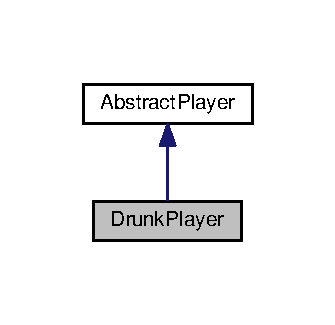
\includegraphics[width=161pt]{classDrunkPlayer__inherit__graph}
\end{center}
\end{figure}


Collaboration diagram for Drunk\+Player\+:\nopagebreak
\begin{figure}[H]
\begin{center}
\leavevmode
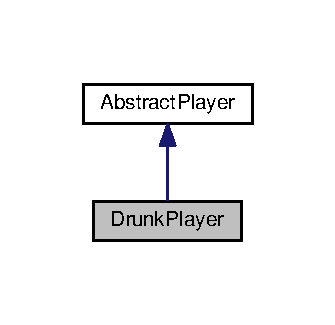
\includegraphics[width=161pt]{classDrunkPlayer__coll__graph}
\end{center}
\end{figure}
\subsection*{Public Member Functions}
\begin{DoxyCompactItemize}
\item 
\hyperlink{classDrunkPlayer_a39c64a774a19456f3a4c194ec5e1131f}{Drunk\+Player} ()
\begin{DoxyCompactList}\small\item\em Constructeur. \end{DoxyCompactList}\item 
void \hyperlink{classDrunkPlayer_a235e60ea8a97c4d26277b066c2cebe80}{load\+Folder} (const std\+::string \&folder\+Name) override
\begin{DoxyCompactList}\small\item\em Lit tous les fichiers d'un dossier. \end{DoxyCompactList}\item 
bool \hyperlink{classDrunkPlayer_a9c032dda7df01fafc757fb1f4e265bb4}{is\+Finished} () const override
\begin{DoxyCompactList}\small\item\em Retourne si toutes les vidéos ont été lues entièrement. \end{DoxyCompactList}\item 
void \hyperlink{classDrunkPlayer_a2662f5010e15c95ca6639f56f012aed1}{operator$>$$>$} (cv\+::\+Mat \&image) override
\begin{DoxyCompactList}\small\item\em Lit une image du flux vidéo. \end{DoxyCompactList}\end{DoxyCompactItemize}
\subsection*{Additional Inherited Members}


\subsection{Detailed Description}
Lecteur vidéo qui lit des vidéos par morceaux désordonnés et transformés. 

\subsection{Constructor \& Destructor Documentation}
\hypertarget{classDrunkPlayer_a39c64a774a19456f3a4c194ec5e1131f}{\index{Drunk\+Player@{Drunk\+Player}!Drunk\+Player@{Drunk\+Player}}
\index{Drunk\+Player@{Drunk\+Player}!Drunk\+Player@{Drunk\+Player}}
\subsubsection[{Drunk\+Player}]{\setlength{\rightskip}{0pt plus 5cm}Drunk\+Player\+::\+Drunk\+Player (
\begin{DoxyParamCaption}
{}
\end{DoxyParamCaption}
)}}\label{classDrunkPlayer_a39c64a774a19456f3a4c194ec5e1131f}


Constructeur. 



\subsection{Member Function Documentation}
\hypertarget{classDrunkPlayer_a9c032dda7df01fafc757fb1f4e265bb4}{\index{Drunk\+Player@{Drunk\+Player}!is\+Finished@{is\+Finished}}
\index{is\+Finished@{is\+Finished}!Drunk\+Player@{Drunk\+Player}}
\subsubsection[{is\+Finished}]{\setlength{\rightskip}{0pt plus 5cm}bool Drunk\+Player\+::is\+Finished (
\begin{DoxyParamCaption}
{}
\end{DoxyParamCaption}
) const\hspace{0.3cm}{\ttfamily [override]}, {\ttfamily [virtual]}}}\label{classDrunkPlayer_a9c032dda7df01fafc757fb1f4e265bb4}


Retourne si toutes les vidéos ont été lues entièrement. 



Implements \hyperlink{classAbstractPlayer_a841896a599ebe6b8317905de78c44bcc}{Abstract\+Player}.

\hypertarget{classDrunkPlayer_a235e60ea8a97c4d26277b066c2cebe80}{\index{Drunk\+Player@{Drunk\+Player}!load\+Folder@{load\+Folder}}
\index{load\+Folder@{load\+Folder}!Drunk\+Player@{Drunk\+Player}}
\subsubsection[{load\+Folder}]{\setlength{\rightskip}{0pt plus 5cm}void Drunk\+Player\+::load\+Folder (
\begin{DoxyParamCaption}
\item[{const std\+::string \&}]{folder\+Name}
\end{DoxyParamCaption}
)\hspace{0.3cm}{\ttfamily [override]}, {\ttfamily [virtual]}}}\label{classDrunkPlayer_a235e60ea8a97c4d26277b066c2cebe80}


Lit tous les fichiers d'un dossier. 



Reimplemented from \hyperlink{classAbstractPlayer_a2091b1757bfd13116dfa4612af55473b}{Abstract\+Player}.

\hypertarget{classDrunkPlayer_a2662f5010e15c95ca6639f56f012aed1}{\index{Drunk\+Player@{Drunk\+Player}!operator$>$$>$@{operator$>$$>$}}
\index{operator$>$$>$@{operator$>$$>$}!Drunk\+Player@{Drunk\+Player}}
\subsubsection[{operator$>$$>$}]{\setlength{\rightskip}{0pt plus 5cm}void Drunk\+Player\+::operator$>$$>$ (
\begin{DoxyParamCaption}
\item[{cv\+::\+Mat \&}]{image}
\end{DoxyParamCaption}
)\hspace{0.3cm}{\ttfamily [override]}, {\ttfamily [virtual]}}}\label{classDrunkPlayer_a2662f5010e15c95ca6639f56f012aed1}


Lit une image du flux vidéo. 



Implements \hyperlink{classAbstractPlayer_a5c9a863c96224dd297aa44c69010cd94}{Abstract\+Player}.



The documentation for this class was generated from the following files\+:\begin{DoxyCompactItemize}
\item 
/etudiants/asmlali/\+G\+L/\+L3\+\_\+\+G\+L\+\_\+etudiant/\+T\+P\+\_\+documentation/drunk\+\_\+player/src/drunk\+\_\+player/\hyperlink{Player_8hpp}{Player.\+hpp}\item 
/etudiants/asmlali/\+G\+L/\+L3\+\_\+\+G\+L\+\_\+etudiant/\+T\+P\+\_\+documentation/drunk\+\_\+player/src/drunk\+\_\+player/\hyperlink{Player_8cpp}{Player.\+cpp}\end{DoxyCompactItemize}

\hypertarget{classRandom}{\section{Random Class Reference}
\label{classRandom}\index{Random@{Random}}
}


{\ttfamily \#include $<$Random.\+hpp$>$}

\subsection*{Public Member Functions}
\begin{DoxyCompactItemize}
\item 
\hyperlink{classRandom_acb76b49c3903a3c4fb67fd216341f08d}{Random} ()
\begin{DoxyCompactList}\small\item\em Constructeur à utiliser. \end{DoxyCompactList}\item 
\hyperlink{classRandom_a9bfadeaa4adc5ac44142d000b1c99441}{Random} (const \hyperlink{classRandom}{Random} \&)=delete
\item 
double \hyperlink{classRandom_aa0277ecffaf7d920b8ebd2399214f113}{operator()} ()
\begin{DoxyCompactList}\small\item\em Génère un nombre aléatoire réel dans \mbox{[}0,1). \end{DoxyCompactList}\item 
int \hyperlink{classRandom_a20265a86364664d85253931dc4685fa3}{operator()} (int n)
\begin{DoxyCompactList}\small\item\em Génère un nombre aléatoire entier dans \mbox{[}0,n). \end{DoxyCompactList}\end{DoxyCompactItemize}


\subsection{Detailed Description}
Générateur de nombre pseudo-\/aléatoire (selon la loi uniforme). Exemple d'utilisation \+: \hyperlink{classRandom}{Random} rng; int x = rng(42); double y = rng(); 

\subsection{Constructor \& Destructor Documentation}
\hypertarget{classRandom_acb76b49c3903a3c4fb67fd216341f08d}{\index{Random@{Random}!Random@{Random}}
\index{Random@{Random}!Random@{Random}}
\subsubsection[{Random}]{\setlength{\rightskip}{0pt plus 5cm}Random\+::\+Random (
\begin{DoxyParamCaption}
{}
\end{DoxyParamCaption}
)}}\label{classRandom_acb76b49c3903a3c4fb67fd216341f08d}


Constructeur à utiliser. 

\hypertarget{classRandom_a9bfadeaa4adc5ac44142d000b1c99441}{\index{Random@{Random}!Random@{Random}}
\index{Random@{Random}!Random@{Random}}
\subsubsection[{Random}]{\setlength{\rightskip}{0pt plus 5cm}Random\+::\+Random (
\begin{DoxyParamCaption}
\item[{const {\bf Random} \&}]{}
\end{DoxyParamCaption}
)\hspace{0.3cm}{\ttfamily [delete]}}}\label{classRandom_a9bfadeaa4adc5ac44142d000b1c99441}
Constructeur par copie interdit. Pour éviter les suites pseudo-\/aléatoires identiques. 

\subsection{Member Function Documentation}
\hypertarget{classRandom_aa0277ecffaf7d920b8ebd2399214f113}{\index{Random@{Random}!operator()@{operator()}}
\index{operator()@{operator()}!Random@{Random}}
\subsubsection[{operator()}]{\setlength{\rightskip}{0pt plus 5cm}double Random\+::operator() (
\begin{DoxyParamCaption}
{}
\end{DoxyParamCaption}
)}}\label{classRandom_aa0277ecffaf7d920b8ebd2399214f113}


Génère un nombre aléatoire réel dans \mbox{[}0,1). 

\hypertarget{classRandom_a20265a86364664d85253931dc4685fa3}{\index{Random@{Random}!operator()@{operator()}}
\index{operator()@{operator()}!Random@{Random}}
\subsubsection[{operator()}]{\setlength{\rightskip}{0pt plus 5cm}int Random\+::operator() (
\begin{DoxyParamCaption}
\item[{int}]{n}
\end{DoxyParamCaption}
)}}\label{classRandom_a20265a86364664d85253931dc4685fa3}


Génère un nombre aléatoire entier dans \mbox{[}0,n). 



The documentation for this class was generated from the following files\+:\begin{DoxyCompactItemize}
\item 
/etudiants/asmlali/\+G\+L/\+L3\+\_\+\+G\+L\+\_\+etudiant/\+T\+P\+\_\+documentation/drunk\+\_\+player/src/drunk\+\_\+player/\hyperlink{Random_8hpp}{Random.\+hpp}\item 
/etudiants/asmlali/\+G\+L/\+L3\+\_\+\+G\+L\+\_\+etudiant/\+T\+P\+\_\+documentation/drunk\+\_\+player/src/drunk\+\_\+player/\hyperlink{Random_8cpp}{Random.\+cpp}\end{DoxyCompactItemize}

\chapter{File Documentation}
\hypertarget{Chrono_8cpp}{\section{/etudiants/asmlali/\+G\+L/\+L3\+\_\+\+G\+L\+\_\+etudiant/\+T\+P\+\_\+documentation/drunk\+\_\+player/src/drunk\+\_\+player/\+Chrono.cpp File Reference}
\label{Chrono_8cpp}\index{/etudiants/asmlali/\+G\+L/\+L3\+\_\+\+G\+L\+\_\+etudiant/\+T\+P\+\_\+documentation/drunk\+\_\+player/src/drunk\+\_\+player/\+Chrono.\+cpp@{/etudiants/asmlali/\+G\+L/\+L3\+\_\+\+G\+L\+\_\+etudiant/\+T\+P\+\_\+documentation/drunk\+\_\+player/src/drunk\+\_\+player/\+Chrono.\+cpp}}
}
{\ttfamily \#include $<$drunk\+\_\+player/\+Chrono.\+hpp$>$}\\*
Include dependency graph for Chrono.\+cpp\+:\nopagebreak
\begin{figure}[H]
\begin{center}
\leavevmode
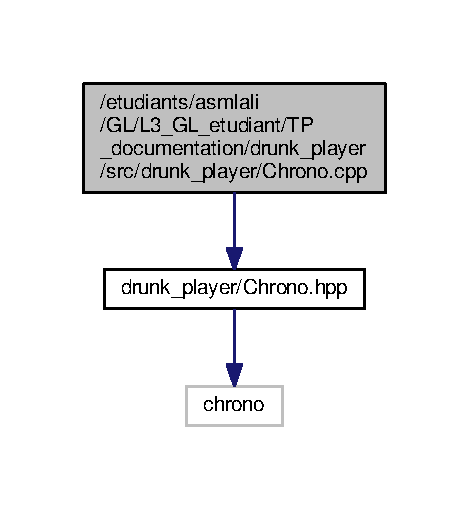
\includegraphics[width=225pt]{Chrono_8cpp__incl}
\end{center}
\end{figure}

\hypertarget{Chrono_8hpp}{\section{/etudiants/asmlali/\+G\+L/\+L3\+\_\+\+G\+L\+\_\+etudiant/\+T\+P\+\_\+documentation/drunk\+\_\+player/src/drunk\+\_\+player/\+Chrono.hpp File Reference}
\label{Chrono_8hpp}\index{/etudiants/asmlali/\+G\+L/\+L3\+\_\+\+G\+L\+\_\+etudiant/\+T\+P\+\_\+documentation/drunk\+\_\+player/src/drunk\+\_\+player/\+Chrono.\+hpp@{/etudiants/asmlali/\+G\+L/\+L3\+\_\+\+G\+L\+\_\+etudiant/\+T\+P\+\_\+documentation/drunk\+\_\+player/src/drunk\+\_\+player/\+Chrono.\+hpp}}
}
{\ttfamily \#include $<$chrono$>$}\\*
Include dependency graph for Chrono.\+hpp\+:\nopagebreak
\begin{figure}[H]
\begin{center}
\leavevmode
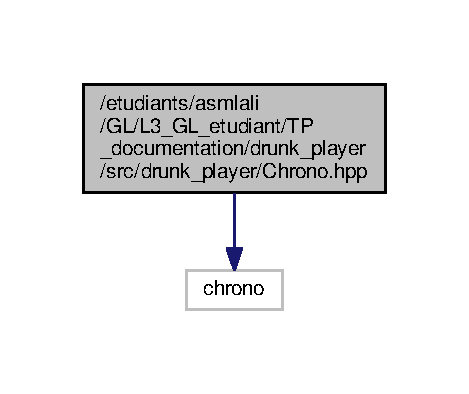
\includegraphics[width=225pt]{Chrono_8hpp__incl}
\end{center}
\end{figure}
This graph shows which files directly or indirectly include this file\+:\nopagebreak
\begin{figure}[H]
\begin{center}
\leavevmode
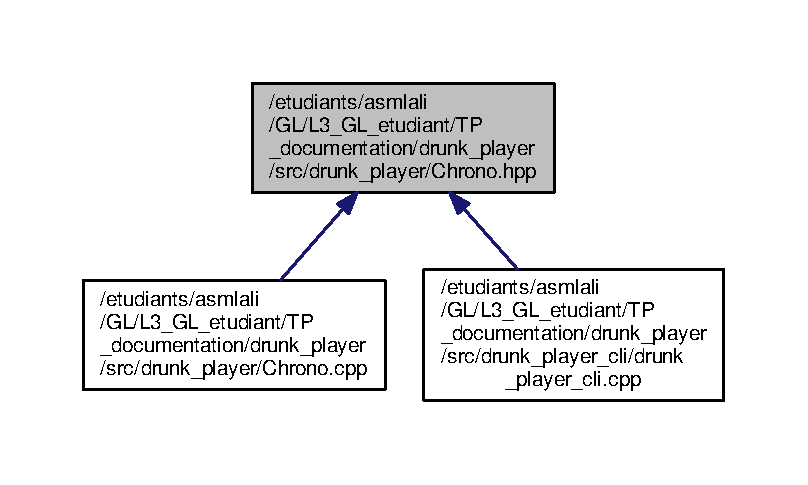
\includegraphics[width=350pt]{Chrono_8hpp__dep__incl}
\end{center}
\end{figure}
\subsection*{Classes}
\begin{DoxyCompactItemize}
\item 
class \hyperlink{classChrono}{Chrono}
\begin{DoxyCompactList}\small\item\em Chronomètre pour mesurer des durées. Exemple d'utilisation \+: \hyperlink{classChrono}{Chrono} chrono; chrono.\+start(); ... chrono.\+stop(); std\+::cout $<$$<$ \char`\"{}temps écoulé \+: \char`\"{} $<$$<$ chrono.\+elapsed() $<$$<$ std\+::endl;. \end{DoxyCompactList}\end{DoxyCompactItemize}

\hypertarget{Filesystem_8cpp}{\section{/etudiants/asmlali/\+G\+L/\+L3\+\_\+\+G\+L\+\_\+etudiant/\+T\+P\+\_\+documentation/drunk\+\_\+player/src/drunk\+\_\+player/\+Filesystem.cpp File Reference}
\label{Filesystem_8cpp}\index{/etudiants/asmlali/\+G\+L/\+L3\+\_\+\+G\+L\+\_\+etudiant/\+T\+P\+\_\+documentation/drunk\+\_\+player/src/drunk\+\_\+player/\+Filesystem.\+cpp@{/etudiants/asmlali/\+G\+L/\+L3\+\_\+\+G\+L\+\_\+etudiant/\+T\+P\+\_\+documentation/drunk\+\_\+player/src/drunk\+\_\+player/\+Filesystem.\+cpp}}
}
{\ttfamily \#include $<$drunk\+\_\+player/\+Filesystem.\+hpp$>$}\\*
{\ttfamily \#include $<$boost/filesystem.\+hpp$>$}\\*
Include dependency graph for Filesystem.\+cpp\+:\nopagebreak
\begin{figure}[H]
\begin{center}
\leavevmode
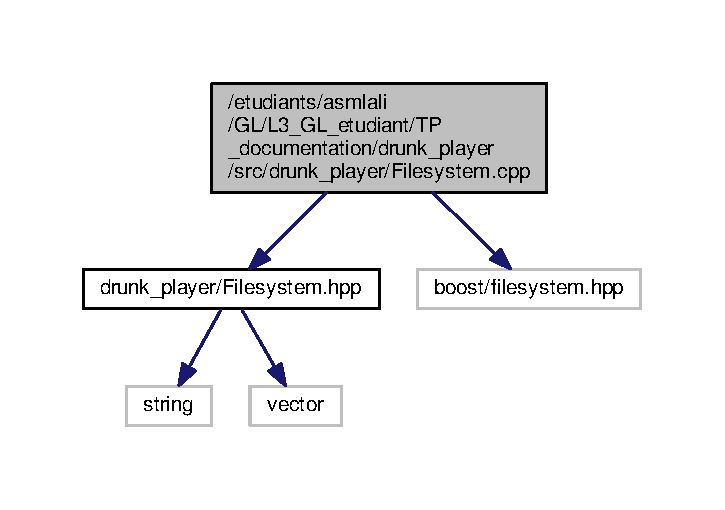
\includegraphics[width=348pt]{Filesystem_8cpp__incl}
\end{center}
\end{figure}
\subsection*{Functions}
\begin{DoxyCompactItemize}
\item 
vector$<$ string $>$ \hyperlink{Filesystem_8cpp_a0bdade166652a07af8445a193dd3f9af}{get\+Files\+In\+Folder} (const string \&pathname)
\end{DoxyCompactItemize}


\subsection{Function Documentation}
\hypertarget{Filesystem_8cpp_a0bdade166652a07af8445a193dd3f9af}{\index{Filesystem.\+cpp@{Filesystem.\+cpp}!get\+Files\+In\+Folder@{get\+Files\+In\+Folder}}
\index{get\+Files\+In\+Folder@{get\+Files\+In\+Folder}!Filesystem.\+cpp@{Filesystem.\+cpp}}
\subsubsection[{get\+Files\+In\+Folder}]{\setlength{\rightskip}{0pt plus 5cm}vector$<$string$>$ get\+Files\+In\+Folder (
\begin{DoxyParamCaption}
\item[{const string \&}]{pathname}
\end{DoxyParamCaption}
)}}\label{Filesystem_8cpp_a0bdade166652a07af8445a193dd3f9af}

\hypertarget{Filesystem_8hpp}{\section{/etudiants/asmlali/\+G\+L/\+L3\+\_\+\+G\+L\+\_\+etudiant/\+T\+P\+\_\+documentation/drunk\+\_\+player/src/drunk\+\_\+player/\+Filesystem.hpp File Reference}
\label{Filesystem_8hpp}\index{/etudiants/asmlali/\+G\+L/\+L3\+\_\+\+G\+L\+\_\+etudiant/\+T\+P\+\_\+documentation/drunk\+\_\+player/src/drunk\+\_\+player/\+Filesystem.\+hpp@{/etudiants/asmlali/\+G\+L/\+L3\+\_\+\+G\+L\+\_\+etudiant/\+T\+P\+\_\+documentation/drunk\+\_\+player/src/drunk\+\_\+player/\+Filesystem.\+hpp}}
}
{\ttfamily \#include $<$string$>$}\\*
{\ttfamily \#include $<$vector$>$}\\*
Include dependency graph for Filesystem.\+hpp\+:\nopagebreak
\begin{figure}[H]
\begin{center}
\leavevmode
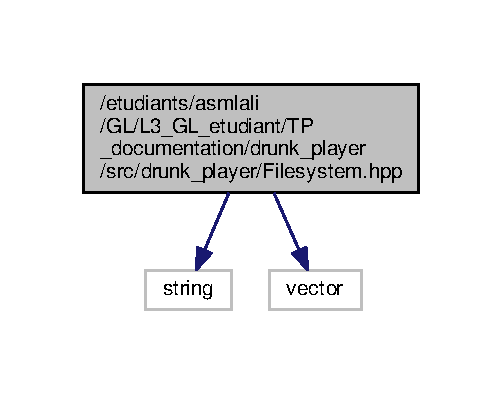
\includegraphics[width=241pt]{Filesystem_8hpp__incl}
\end{center}
\end{figure}
This graph shows which files directly or indirectly include this file\+:\nopagebreak
\begin{figure}[H]
\begin{center}
\leavevmode
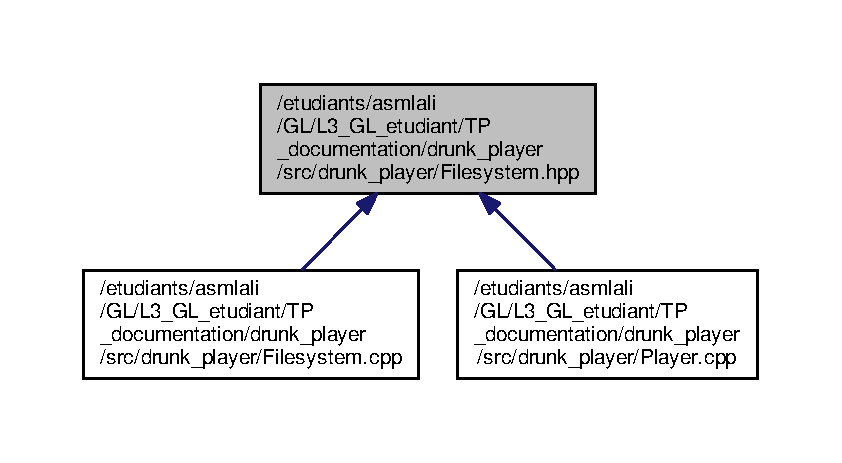
\includegraphics[width=350pt]{Filesystem_8hpp__dep__incl}
\end{center}
\end{figure}
\subsection*{Functions}
\begin{DoxyCompactItemize}
\item 
std\+::vector$<$ std\+::string $>$ \hyperlink{Filesystem_8hpp_a40a3f80a49c54ab8ddcb4c2d2fe6d384}{get\+Files\+In\+Folder} (const std\+::string \&pathname)
\end{DoxyCompactItemize}


\subsection{Function Documentation}
\hypertarget{Filesystem_8hpp_a40a3f80a49c54ab8ddcb4c2d2fe6d384}{\index{Filesystem.\+hpp@{Filesystem.\+hpp}!get\+Files\+In\+Folder@{get\+Files\+In\+Folder}}
\index{get\+Files\+In\+Folder@{get\+Files\+In\+Folder}!Filesystem.\+hpp@{Filesystem.\+hpp}}
\subsubsection[{get\+Files\+In\+Folder}]{\setlength{\rightskip}{0pt plus 5cm}std\+::vector$<$std\+::string$>$ get\+Files\+In\+Folder (
\begin{DoxyParamCaption}
\item[{const std\+::string \&}]{pathname}
\end{DoxyParamCaption}
)}}\label{Filesystem_8hpp_a40a3f80a49c54ab8ddcb4c2d2fe6d384}
Retourne la liste des fichiers contenus dans un dossier. Les fichiers sont donnés avec leur chemin relatif. 
\hypertarget{Player_8cpp}{\section{/etudiants/asmlali/\+G\+L/\+L3\+\_\+\+G\+L\+\_\+etudiant/\+T\+P\+\_\+documentation/drunk\+\_\+player/src/drunk\+\_\+player/\+Player.cpp File Reference}
\label{Player_8cpp}\index{/etudiants/asmlali/\+G\+L/\+L3\+\_\+\+G\+L\+\_\+etudiant/\+T\+P\+\_\+documentation/drunk\+\_\+player/src/drunk\+\_\+player/\+Player.\+cpp@{/etudiants/asmlali/\+G\+L/\+L3\+\_\+\+G\+L\+\_\+etudiant/\+T\+P\+\_\+documentation/drunk\+\_\+player/src/drunk\+\_\+player/\+Player.\+cpp}}
}
{\ttfamily \#include $<$drunk\+\_\+player/\+Player.\+hpp$>$}\\*
{\ttfamily \#include $<$drunk\+\_\+player/\+Filesystem.\+hpp$>$}\\*
Include dependency graph for Player.\+cpp\+:\nopagebreak
\begin{figure}[H]
\begin{center}
\leavevmode
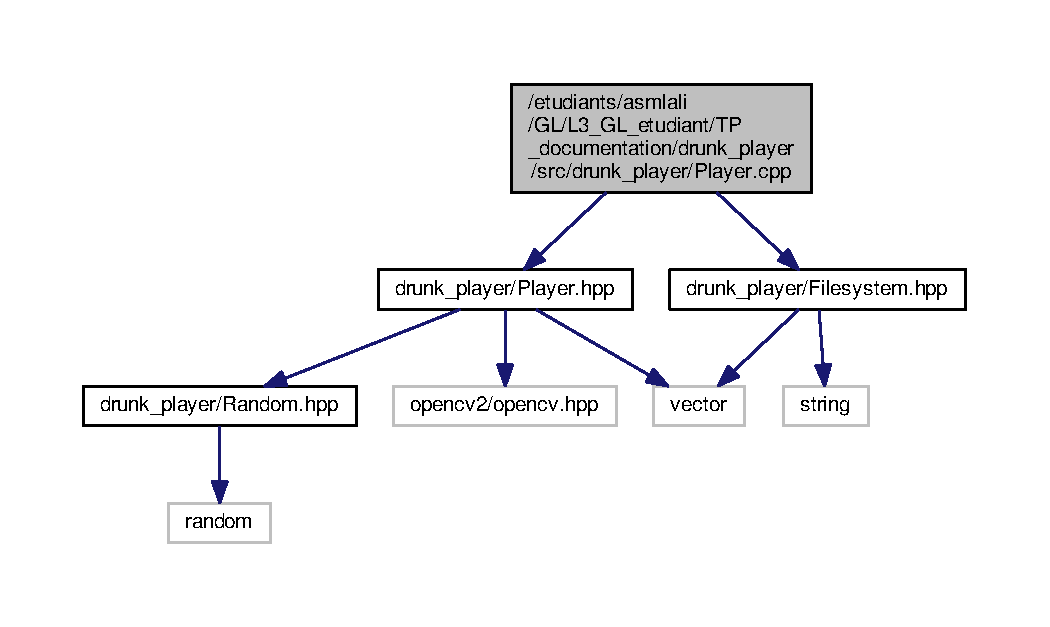
\includegraphics[width=350pt]{Player_8cpp__incl}
\end{center}
\end{figure}

\hypertarget{Player_8hpp}{\section{/etudiants/asmlali/\+G\+L/\+L3\+\_\+\+G\+L\+\_\+etudiant/\+T\+P\+\_\+documentation/drunk\+\_\+player/src/drunk\+\_\+player/\+Player.hpp File Reference}
\label{Player_8hpp}\index{/etudiants/asmlali/\+G\+L/\+L3\+\_\+\+G\+L\+\_\+etudiant/\+T\+P\+\_\+documentation/drunk\+\_\+player/src/drunk\+\_\+player/\+Player.\+hpp@{/etudiants/asmlali/\+G\+L/\+L3\+\_\+\+G\+L\+\_\+etudiant/\+T\+P\+\_\+documentation/drunk\+\_\+player/src/drunk\+\_\+player/\+Player.\+hpp}}
}
{\ttfamily \#include $<$drunk\+\_\+player/\+Random.\+hpp$>$}\\*
{\ttfamily \#include $<$opencv2/opencv.\+hpp$>$}\\*
{\ttfamily \#include $<$vector$>$}\\*
Include dependency graph for Player.\+hpp\+:\nopagebreak
\begin{figure}[H]
\begin{center}
\leavevmode
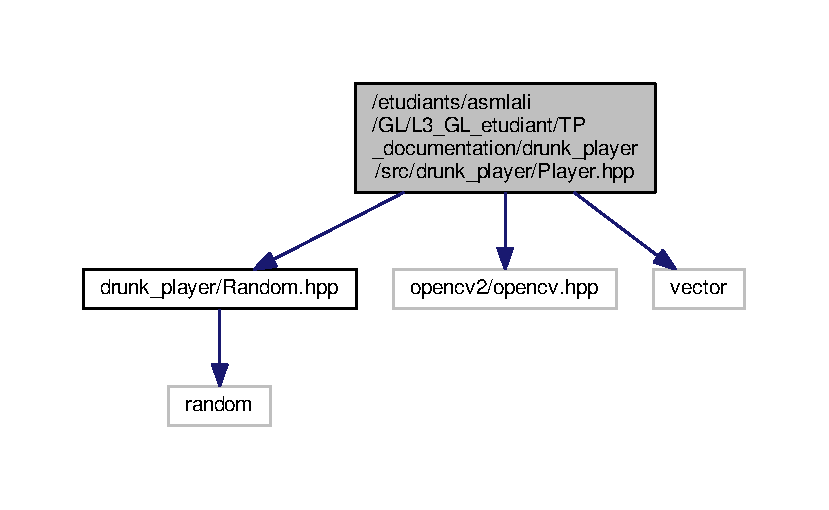
\includegraphics[width=350pt]{Player_8hpp__incl}
\end{center}
\end{figure}
This graph shows which files directly or indirectly include this file\+:\nopagebreak
\begin{figure}[H]
\begin{center}
\leavevmode
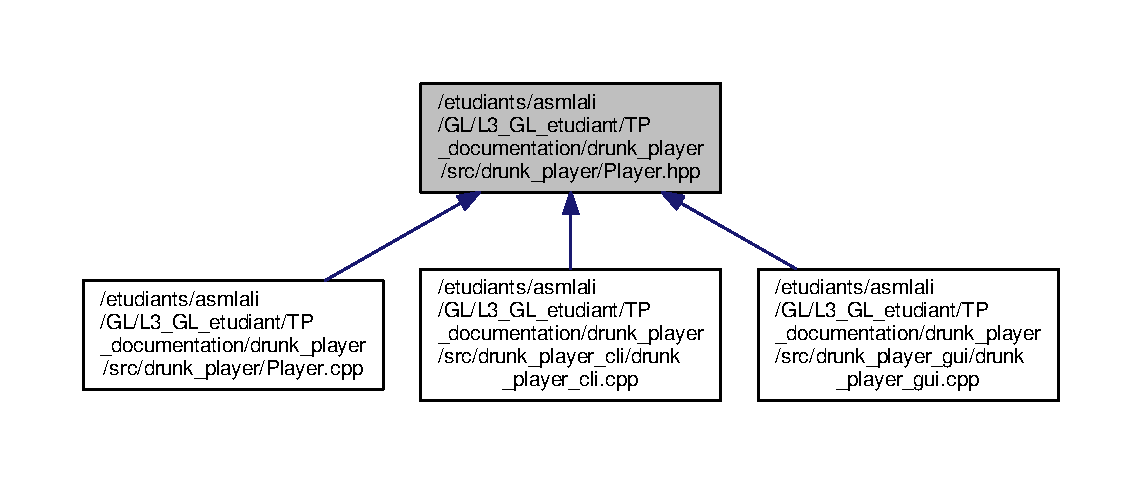
\includegraphics[width=350pt]{Player_8hpp__dep__incl}
\end{center}
\end{figure}
\subsection*{Classes}
\begin{DoxyCompactItemize}
\item 
class \hyperlink{classAbstractPlayer}{Abstract\+Player}
\item 
class \hyperlink{classDrunkPlayer}{Drunk\+Player}
\begin{DoxyCompactList}\small\item\em Lecteur vidéo qui lit des vidéos par morceaux désordonnés et transformés. \end{DoxyCompactList}\end{DoxyCompactItemize}

\hypertarget{Random_8cpp}{\section{/etudiants/asmlali/\+G\+L/\+L3\+\_\+\+G\+L\+\_\+etudiant/\+T\+P\+\_\+documentation/drunk\+\_\+player/src/drunk\+\_\+player/\+Random.cpp File Reference}
\label{Random_8cpp}\index{/etudiants/asmlali/\+G\+L/\+L3\+\_\+\+G\+L\+\_\+etudiant/\+T\+P\+\_\+documentation/drunk\+\_\+player/src/drunk\+\_\+player/\+Random.\+cpp@{/etudiants/asmlali/\+G\+L/\+L3\+\_\+\+G\+L\+\_\+etudiant/\+T\+P\+\_\+documentation/drunk\+\_\+player/src/drunk\+\_\+player/\+Random.\+cpp}}
}
{\ttfamily \#include $<$drunk\+\_\+player/\+Random.\+hpp$>$}\\*
Include dependency graph for Random.\+cpp\+:\nopagebreak
\begin{figure}[H]
\begin{center}
\leavevmode
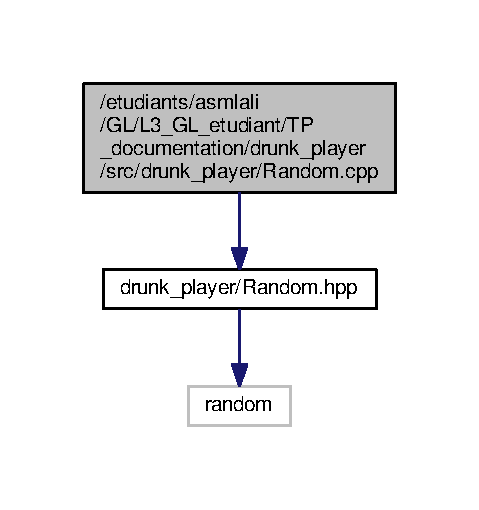
\includegraphics[width=230pt]{Random_8cpp__incl}
\end{center}
\end{figure}

\hypertarget{Random_8hpp}{\section{/etudiants/asmlali/\+G\+L/\+L3\+\_\+\+G\+L\+\_\+etudiant/\+T\+P\+\_\+documentation/drunk\+\_\+player/src/drunk\+\_\+player/\+Random.hpp File Reference}
\label{Random_8hpp}\index{/etudiants/asmlali/\+G\+L/\+L3\+\_\+\+G\+L\+\_\+etudiant/\+T\+P\+\_\+documentation/drunk\+\_\+player/src/drunk\+\_\+player/\+Random.\+hpp@{/etudiants/asmlali/\+G\+L/\+L3\+\_\+\+G\+L\+\_\+etudiant/\+T\+P\+\_\+documentation/drunk\+\_\+player/src/drunk\+\_\+player/\+Random.\+hpp}}
}
{\ttfamily \#include $<$random$>$}\\*
Include dependency graph for Random.\+hpp\+:\nopagebreak
\begin{figure}[H]
\begin{center}
\leavevmode
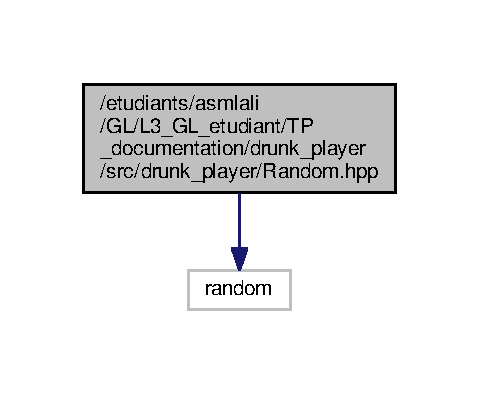
\includegraphics[width=230pt]{Random_8hpp__incl}
\end{center}
\end{figure}
This graph shows which files directly or indirectly include this file\+:\nopagebreak
\begin{figure}[H]
\begin{center}
\leavevmode
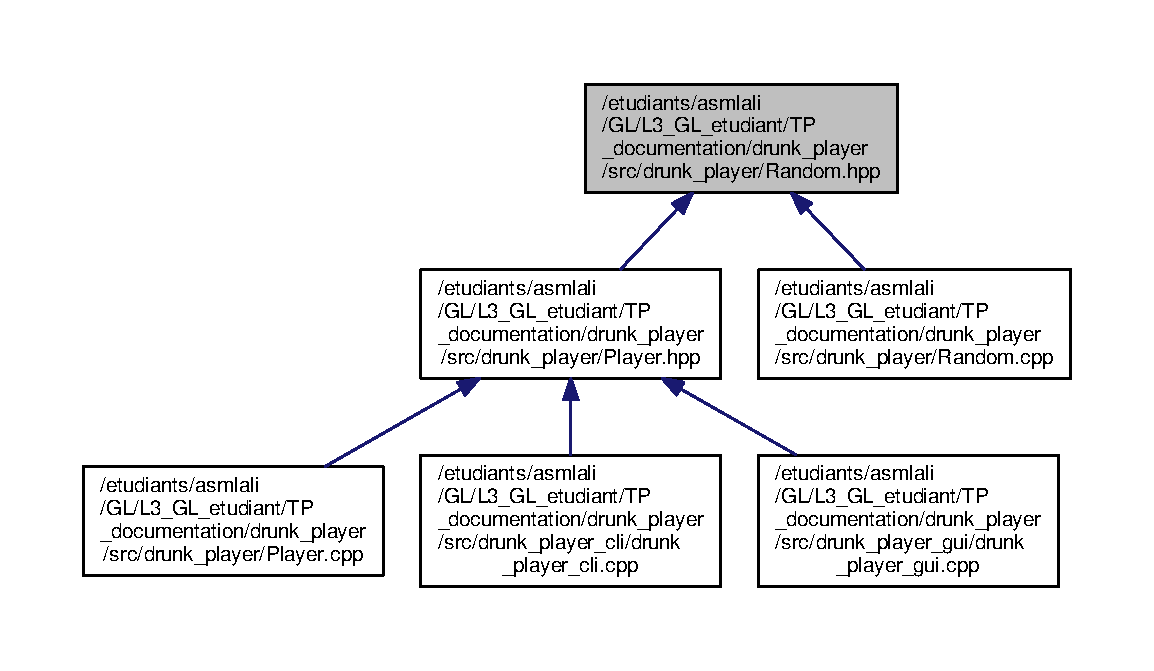
\includegraphics[width=350pt]{Random_8hpp__dep__incl}
\end{center}
\end{figure}
\subsection*{Classes}
\begin{DoxyCompactItemize}
\item 
class \hyperlink{classRandom}{Random}
\end{DoxyCompactItemize}

\hypertarget{drunk__player__cli_8cpp}{\section{/etudiants/asmlali/\+G\+L/\+L3\+\_\+\+G\+L\+\_\+etudiant/\+T\+P\+\_\+documentation/drunk\+\_\+player/src/drunk\+\_\+player\+\_\+cli/drunk\+\_\+player\+\_\+cli.cpp File Reference}
\label{drunk__player__cli_8cpp}\index{/etudiants/asmlali/\+G\+L/\+L3\+\_\+\+G\+L\+\_\+etudiant/\+T\+P\+\_\+documentation/drunk\+\_\+player/src/drunk\+\_\+player\+\_\+cli/drunk\+\_\+player\+\_\+cli.\+cpp@{/etudiants/asmlali/\+G\+L/\+L3\+\_\+\+G\+L\+\_\+etudiant/\+T\+P\+\_\+documentation/drunk\+\_\+player/src/drunk\+\_\+player\+\_\+cli/drunk\+\_\+player\+\_\+cli.\+cpp}}
}
{\ttfamily \#include $<$drunk\+\_\+player/\+Chrono.\+hpp$>$}\\*
{\ttfamily \#include $<$drunk\+\_\+player/\+Player.\+hpp$>$}\\*
{\ttfamily \#include $<$iostream$>$}\\*
Include dependency graph for drunk\+\_\+player\+\_\+cli.\+cpp\+:\nopagebreak
\begin{figure}[H]
\begin{center}
\leavevmode
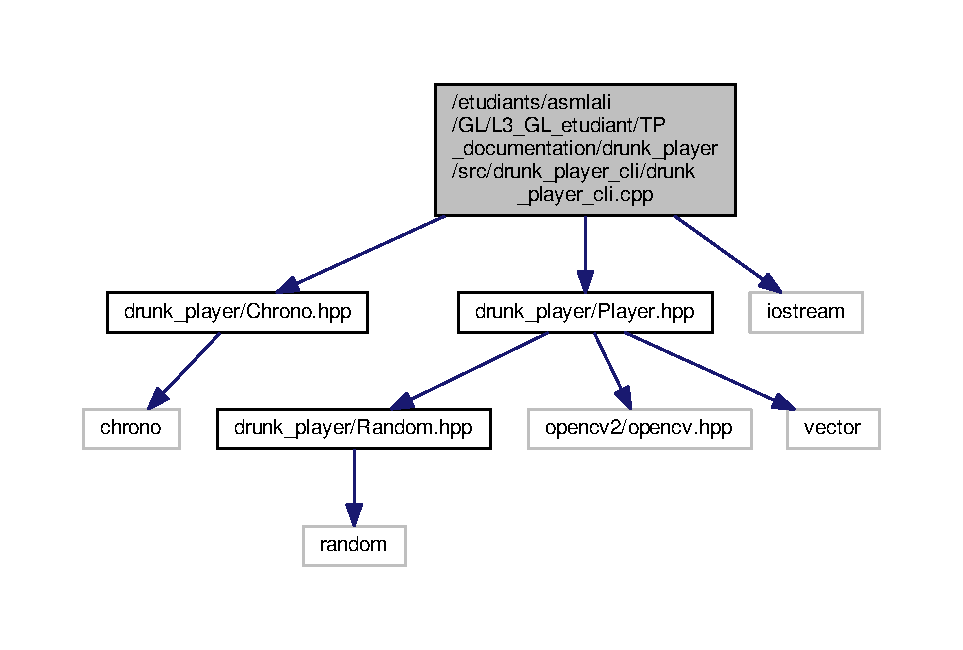
\includegraphics[width=350pt]{drunk__player__cli_8cpp__incl}
\end{center}
\end{figure}
\subsection*{Functions}
\begin{DoxyCompactItemize}
\item 
int \hyperlink{drunk__player__cli_8cpp_a3c04138a5bfe5d72780bb7e82a18e627}{main} (int argc, char $\ast$$\ast$argv)
\end{DoxyCompactItemize}


\subsection{Function Documentation}
\hypertarget{drunk__player__cli_8cpp_a3c04138a5bfe5d72780bb7e82a18e627}{\index{drunk\+\_\+player\+\_\+cli.\+cpp@{drunk\+\_\+player\+\_\+cli.\+cpp}!main@{main}}
\index{main@{main}!drunk\+\_\+player\+\_\+cli.\+cpp@{drunk\+\_\+player\+\_\+cli.\+cpp}}
\subsubsection[{main}]{\setlength{\rightskip}{0pt plus 5cm}int main (
\begin{DoxyParamCaption}
\item[{int}]{argc, }
\item[{char $\ast$$\ast$}]{argv}
\end{DoxyParamCaption}
)}}\label{drunk__player__cli_8cpp_a3c04138a5bfe5d72780bb7e82a18e627}

\hypertarget{drunk__player__gui_8cpp}{\section{/etudiants/asmlali/\+G\+L/\+L3\+\_\+\+G\+L\+\_\+etudiant/\+T\+P\+\_\+documentation/drunk\+\_\+player/src/drunk\+\_\+player\+\_\+gui/drunk\+\_\+player\+\_\+gui.cpp File Reference}
\label{drunk__player__gui_8cpp}\index{/etudiants/asmlali/\+G\+L/\+L3\+\_\+\+G\+L\+\_\+etudiant/\+T\+P\+\_\+documentation/drunk\+\_\+player/src/drunk\+\_\+player\+\_\+gui/drunk\+\_\+player\+\_\+gui.\+cpp@{/etudiants/asmlali/\+G\+L/\+L3\+\_\+\+G\+L\+\_\+etudiant/\+T\+P\+\_\+documentation/drunk\+\_\+player/src/drunk\+\_\+player\+\_\+gui/drunk\+\_\+player\+\_\+gui.\+cpp}}
}
{\ttfamily \#include $<$drunk\+\_\+player/\+Player.\+hpp$>$}\\*
{\ttfamily \#include $<$iostream$>$}\\*
Include dependency graph for drunk\+\_\+player\+\_\+gui.\+cpp\+:\nopagebreak
\begin{figure}[H]
\begin{center}
\leavevmode
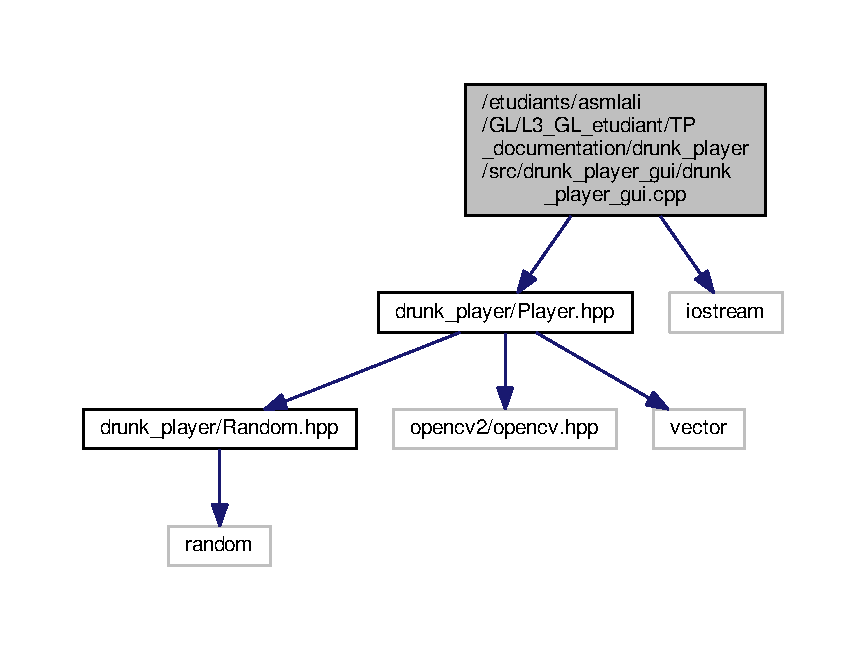
\includegraphics[width=350pt]{drunk__player__gui_8cpp__incl}
\end{center}
\end{figure}
\subsection*{Functions}
\begin{DoxyCompactItemize}
\item 
int \hyperlink{drunk__player__gui_8cpp_a3c04138a5bfe5d72780bb7e82a18e627}{main} (int argc, char $\ast$$\ast$argv)
\end{DoxyCompactItemize}


\subsection{Function Documentation}
\hypertarget{drunk__player__gui_8cpp_a3c04138a5bfe5d72780bb7e82a18e627}{\index{drunk\+\_\+player\+\_\+gui.\+cpp@{drunk\+\_\+player\+\_\+gui.\+cpp}!main@{main}}
\index{main@{main}!drunk\+\_\+player\+\_\+gui.\+cpp@{drunk\+\_\+player\+\_\+gui.\+cpp}}
\subsubsection[{main}]{\setlength{\rightskip}{0pt plus 5cm}int main (
\begin{DoxyParamCaption}
\item[{int}]{argc, }
\item[{char $\ast$$\ast$}]{argv}
\end{DoxyParamCaption}
)}}\label{drunk__player__gui_8cpp_a3c04138a5bfe5d72780bb7e82a18e627}

\hypertarget{mainpage_8hpp}{\section{/etudiants/asmlali/\+G\+L/\+L3\+\_\+\+G\+L\+\_\+etudiant/\+T\+P\+\_\+documentation/drunk\+\_\+player/src/mainpage.hpp File Reference}
\label{mainpage_8hpp}\index{/etudiants/asmlali/\+G\+L/\+L3\+\_\+\+G\+L\+\_\+etudiant/\+T\+P\+\_\+documentation/drunk\+\_\+player/src/mainpage.\+hpp@{/etudiants/asmlali/\+G\+L/\+L3\+\_\+\+G\+L\+\_\+etudiant/\+T\+P\+\_\+documentation/drunk\+\_\+player/src/mainpage.\+hpp}}
}

%--- End generated contents ---

% Index
\newpage
\phantomsection
\addcontentsline{toc}{chapter}{Index}
\printindex

\end{document}
